% !TeX spellcheck = en_US
% !TEX root = ../thesis-example.tex
%
\chapter{Extending Reality}
\label{sec:extendingreality}

\cleanchapterquote{You are an aperture through which the universe is looking at 
and exploring itself.}{Alan W. Watts}{(Philosopher)}

The well known urban legend of "L'Arriv\'ee d'un train en gare de La Ciotat" in 
which a train arrives at the La Ciotat station, is, that "the audience was so 
overwhelmed by the moving image [...] coming directly at them that people 
screamed and ran to the back of the room". \cite{wiki:train:2017} With that a 
new medium was born, which matured into a new art form of film and movies.
\newline
Most important is that with this short clip opened a door beyond still images 
and their limited depiction of motion. Video imagery changed our imagination 
and allowed for a new communication form, inviting into an animated, moving 
world. There have been great achievements in the last century in motion video 
production with a great amount of visual trickery for composing more realistic 
and imaginative video content. With the help of Computer Generated Imagery 
(CGI) blurs the boundaries between real acting and virtual recreation so very 
far, that it is almost impossible to differentiate between real world video 
capture and 3D recreated imagery.

\section{Motion Video Production}

Producing motion video has come a long way and a sufficient history of it would 
be far out of scope for this thesis. Concentrating on key aspects of 
composition techniques might give an appropriate overview to range where Mixed 
Reality takes its inspiration from.

Way before digital imaging processing took over production sets similar 
problems as discussed in this thesis had to be solved, i. e. how an actor can 
be captured without a back- or foreground and how he would then be integrated 
into an imaginative set. Today, modern action movies don't even necessarily 
capture the actor but his movements, which then will be artificially rendered 
with computer generated imagery.

\todo[inline]{Missing: Camera tricks, computer aided visual effects, green 
screens}

\section{CGI \& Video Composition}

\subsection{History of Green \& Blue Screen Productions}

Set theory is beyond the scope of this thesis, but green- and blue screen 
production has first and foremost a simple reasoning: Green and blue are two of 
the three color triplets that resemble a least amount of color found in 
capturing of humans - and to a certain extent any flora and fauna. Since chroma 
keying (see Ch. \ref{sec:chromakey}) takes color distance as general basis, 
production environments generally use green screen keying.
\newline
Green boxes abuse a correlating advantage that the human eye is most 
susceptible to green, allowing for a visual high color range and an ability to 
differentiate between many shades of green. Experiments to color range have 
been done since 1942, trying to understand gambit ranges and color 
differentiation of human vision. Experiments concluded that eye cone cells see 
a blending range of wavelengths to different intensities, giving the green 
vector space its highest perceptible range. \cite{MacAdam:1942}

\begin{figure}[htbp]
	\label{fig:greenscreen:stimula}
	\begin{subfigure}[t]{.35\textwidth}
		\centering
		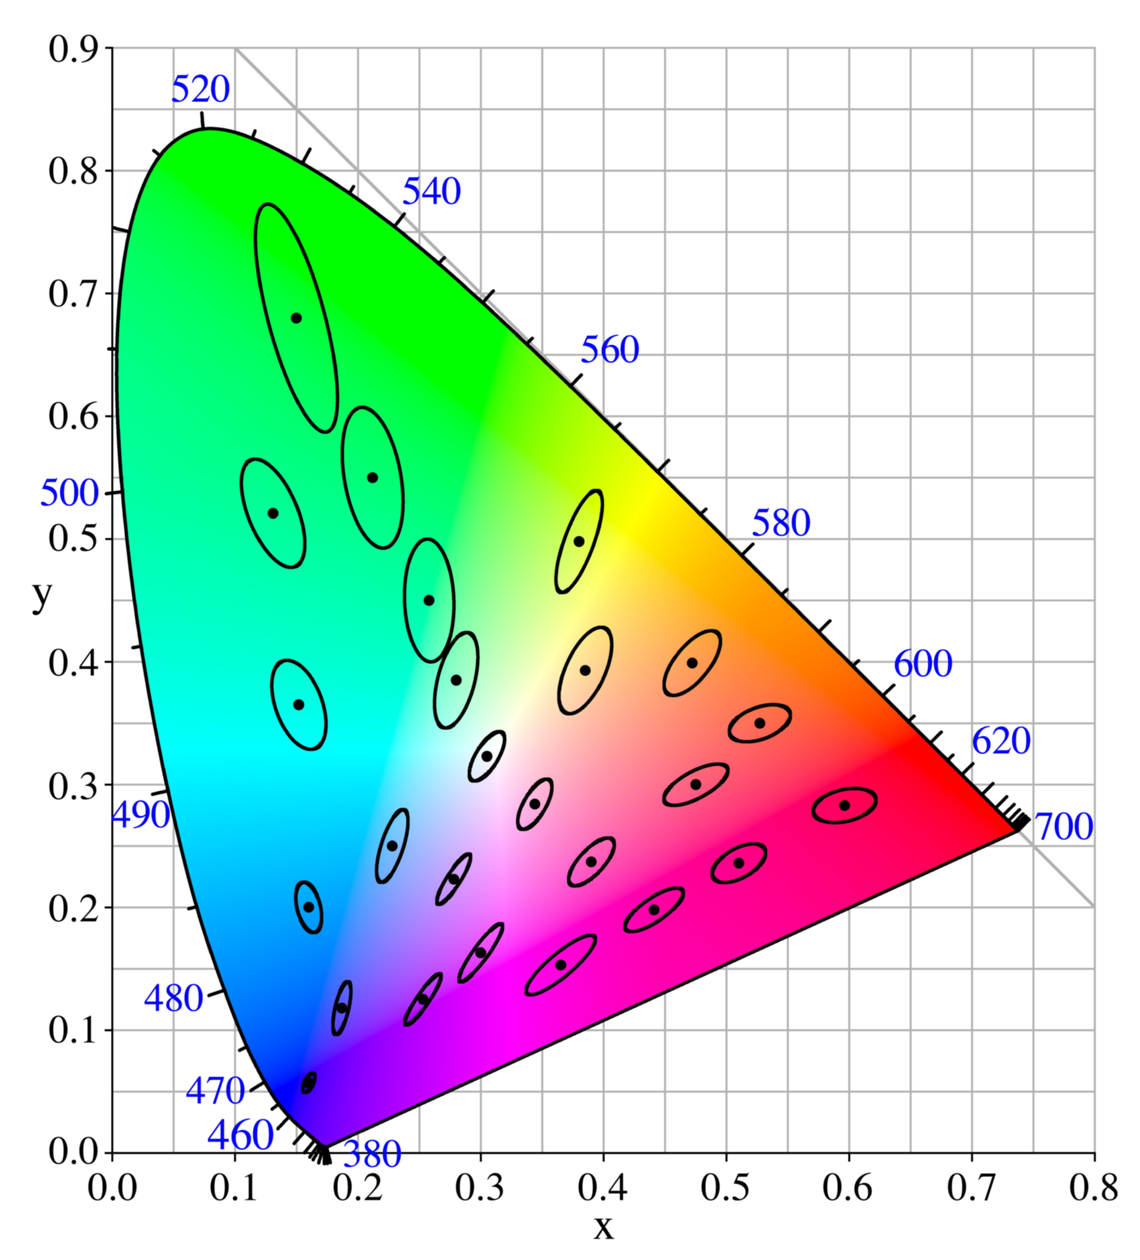
\includegraphics[width=\textwidth]{_external/media/CIExy1931_MacAdam.png}
	\caption{MacAdam ellipses on 1931 standard chromaticity diagram 
		\cite{wiki:macadam:2017}}
	\end{subfigure}
	\begin{subfigure}[t]{.5\textwidth}
		\centering
		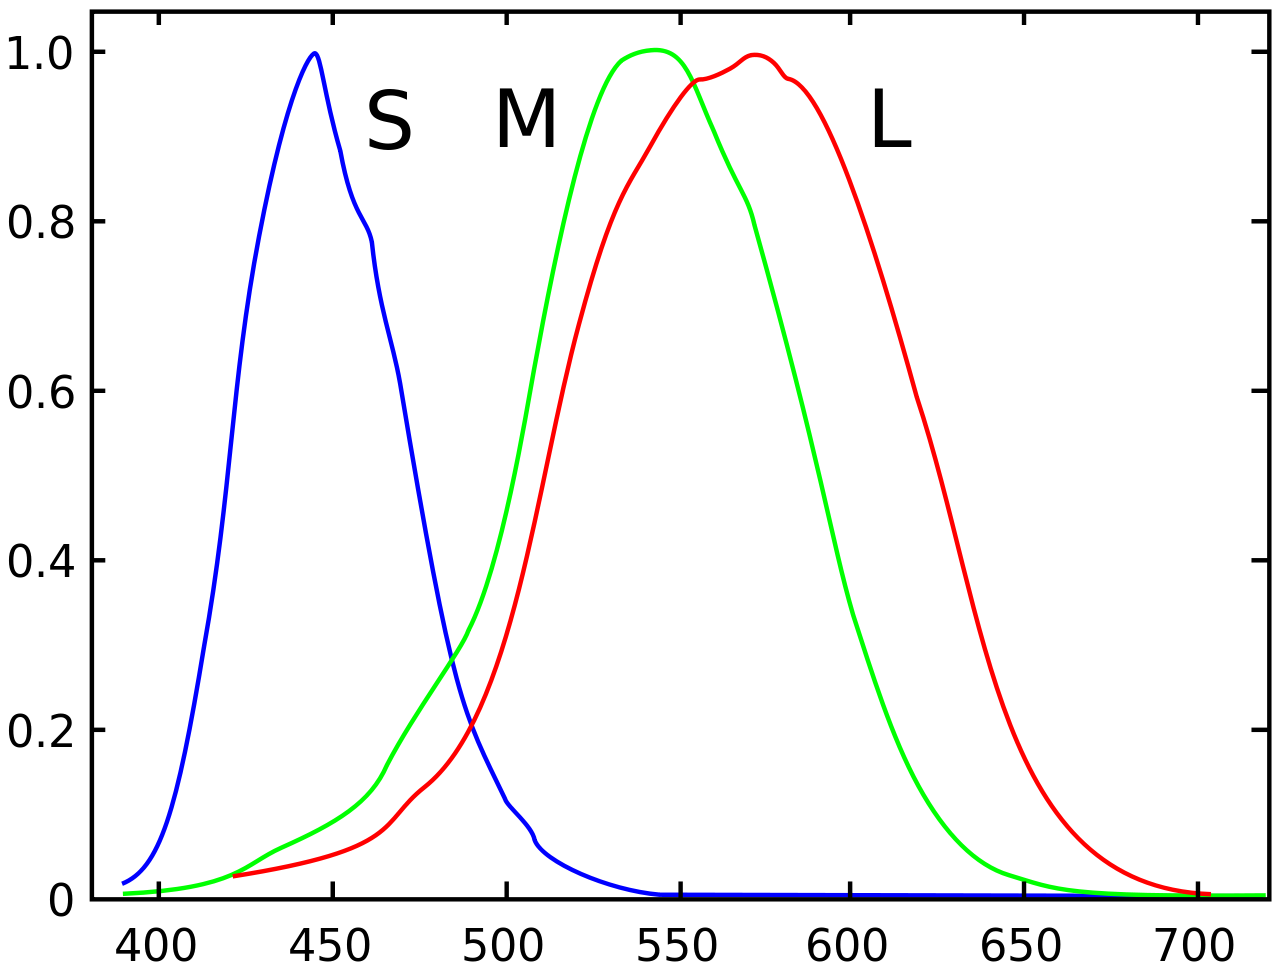
\includegraphics[width=\textwidth]{_external/media/1280px-Cones_SMJ2_E.png}
		\caption{Normalized responsivity spectra of human cone cells, S, M, and 
		L types after Wyszecki et. al \cite{wiki:Wyszecki:2017}}. Notice the 
		overlap between M and L cones.
	\end{subfigure}
\end{figure}

\todo[inline]{The layout is a bit wonky here.}

Most consumer cameras - and even most production cameras - use dot-matrix 
sensors with a weighted ration of green (4), red (2) and blue (2) pixels, 
called Bayer pattern \cite{kodak:bayer:1976}. Green is generally easier to 
light, illuminate and adjust over blue screens. Small irregularities, for 
example through uneven lightning or crinkles in the material, can be adjusted 
easily by the user and allows for a relatively clean camera image generation.
\newline
The quality of input footage makes a big difference in separating back- and 
foreground, hence is a well lit and adjusted set a good backbone for well 
working chroma keying.

\section{What's VR - Differentiation of AR, VR \& MR}

In search of an appropriate abbreviation for computer-enhanced realtime imagery 
a recent addition is "XR", where \textit{X} is a letter of your choice. 
Definitions are getting more diluted and generally describe a technique, rather 
than an apparent effect by now.

\begin{figure}[htb]
	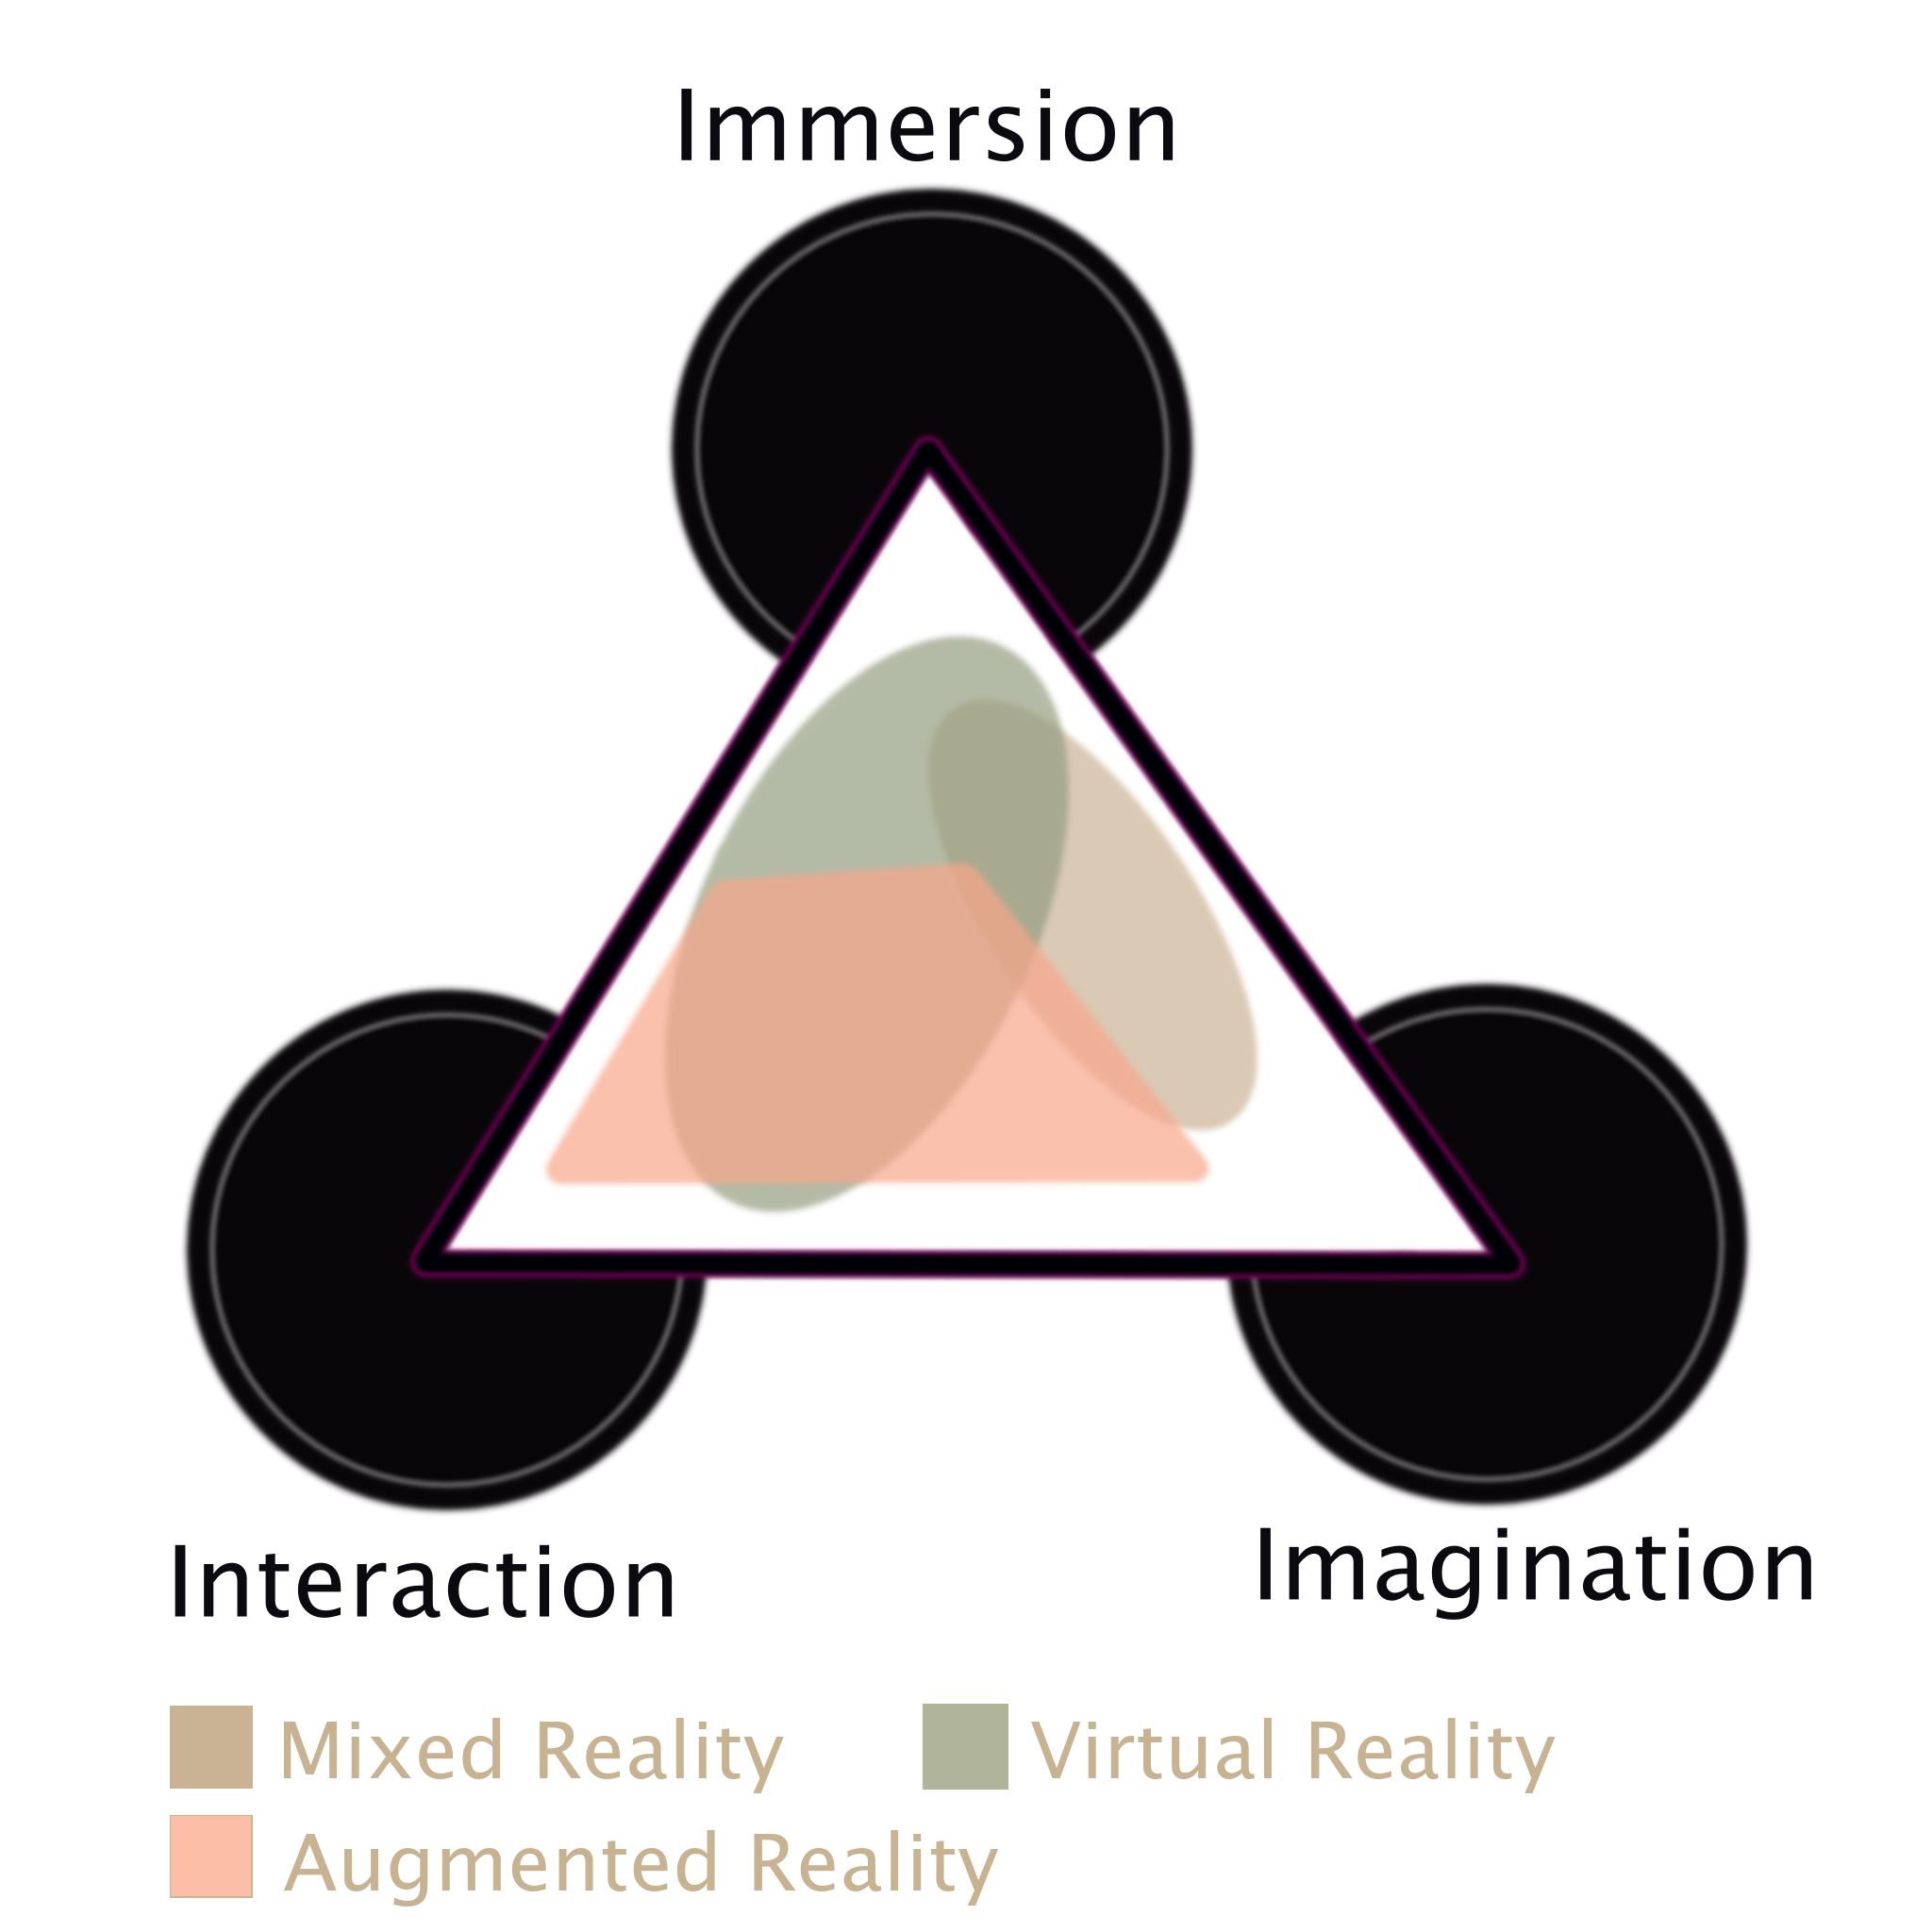
\includegraphics[width=\textwidth]{_raw_resources/i3-triangle.png}
	\caption{I\textsuperscript{3} Triangle - figurative quantization of 
		different reality extending methods}
	\label{fig:xr:i3-triangle}
\end{figure}
Augmented Reality (AR) is a concept by augmenting real world imagery with 
additional information and interactable objects. It ranges from very simple 
devices displaying data in the field of view of a user up to full augmentation, 
displaying 3D models overlaying on real world objects. This can be done ranging 
from Pepper's Ghost projections, augmenting video - a famous example is the 
rather successful "Pokémon GO" -, up to the Microsoft HoloLens, that has 
sensors for a wide range of spatial mapping, spatial anchoring and distance 
field calculation.

Virtual Reality is a concept usually done by stereo projection of a 3D 
environment inside a Head Mounted Display. It takes an user out of the current 
room and sets him into a complete new, virtual reality - hence it's names 
origin. HMD hardware ranges from the simplistic Google Cardboard 
\footnote{using a smartphone as display device} to the Samsung GearVR 
\footnote{similarly uses a smartphone as display driver} up to the Oculus Rift 
and HTC Vive. The latter two products offer room-scale experiences where a user 
is able to move freely in his play space (basically a tacked bounding volume) 
and allows for six degrees of freedom (\gls{6dof}) tracking.

Mixed Reality is an extension of Virtual Reality, allowing bystanders to get an 
impression of the virtual reality around an actor. By reproducing virtual 
projection parameters of a 3D environment, it is possible to place a real world 
camera feed at the right position inside the 3D application. This yields to a 
combined technique of Augmented and Virtual Reality. A production environment 
can be achieved with a \gls{6DOF} HMD and additional - either user- or tracking 
input of - positional parameters for the camera. 

\section{Immersion vs. Communication}

\todo[inline]{maybe the overview does already a "good enough" job to bring this 
across.}

Virtual Reality, as previously mentioned in \ref{sec:intro:outline}, is very 
immersive but the experience is hard to imagine without wearing a HMD yourself. 
Additionally doesn't VR offer any ways to allow observers a similar experience 
as the VR actor.
\newline
A very obvious problem starts on interaction. A VR user doesn't always need to 
see his hands to interact with a scene, due to the natural way of holding these 
controllers in his hands and directly translating controller interaction to the
virtual environment. An outside viewer however does not see hands and will 
not understand actions performed by the user if he cannot see the virtual 
hands. Any usage context that happens off-screen cannot be communicated and 
will be therefore lost.
\newline
A recent game example, Rick and Morty: Virtual Rick-ality, tries to mitigate 
this issue by placing virtual CCTV cameras into the scene, which can be 
controlled through outside viewers - giving a neutral third-person view into 
the three-dimension scene. The VR actor is replaced as a loose avatar 
representing a figure (Morty) from the cartoons universe.

\todo[inline]{Add a screenshot of that}

Mixed Reality merges the actors and virtual realities context, allowing outside 
bystanders a comparable window into the actors experienced world. In fact, 
initial promotional material for the HTC Vive showed mixed reality footage, 
produced by one VR computer and a secondary composition PC 
\cite{valve:mr-production:2016}. It's setup is comparable to the one in this 
thesis and differs by using more than one software context, done by outputting 
a rendered image of the virtual scene and compositing it on another system.

\subsection{Evolution of Virtual Reality Footage}

Originally footage consisted of the output that was sent to the headset, 
including image transformation that needs to be done to correct the headset 
lenses \footnote{this is referred to as "Barrel Distortion"} - this distorted 
dual image is very hard to follow, as it adds two ambiguous images and has 
additional a high distortion. Since the direct feed to a HMD is used, any 
translation of the headsets position is visible, which results in a jittery 
motion feed.

\begin{figure}[htbp]
	\label{fig:evolution:steps}
	\begin{subfigure}[t]{.45\textwidth}
		\centering
		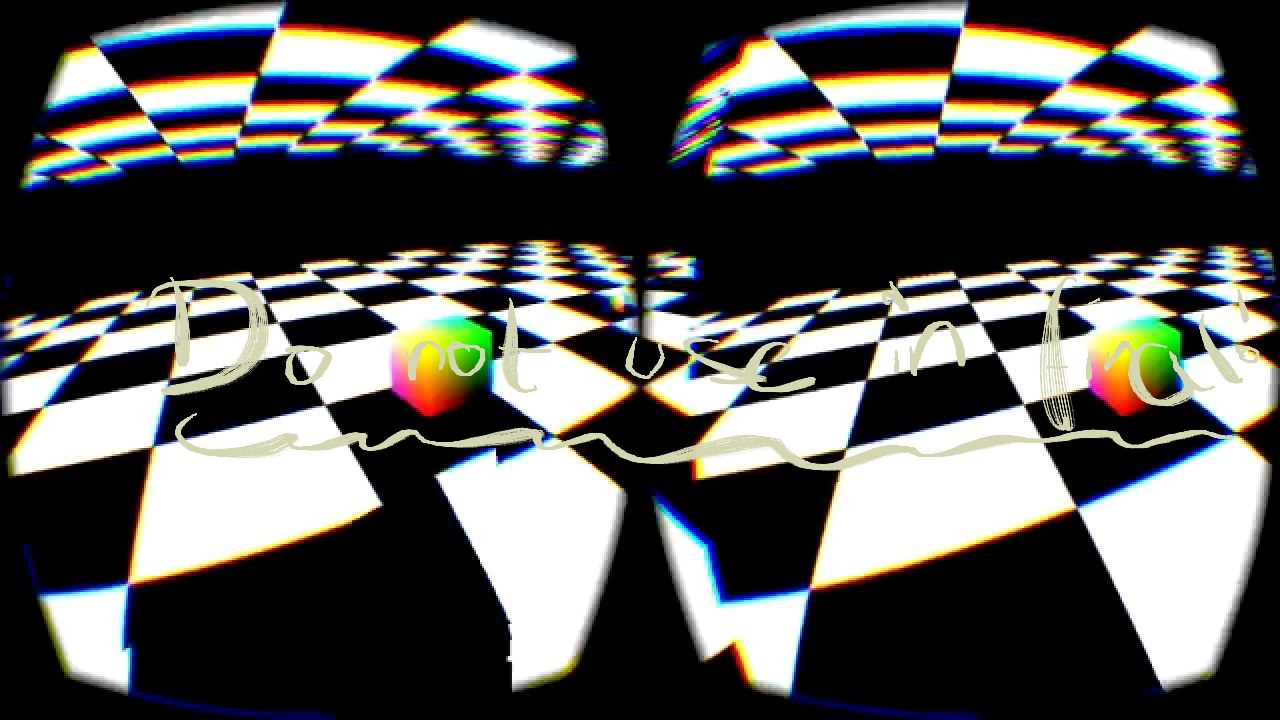
\includegraphics[width=\textwidth]{_raw_resources/lens_distortion.jpeg}
		\caption{Distorted direct dual output to a Oculus DK2.}
	\end{subfigure}
	\begin{subfigure}[t]{.45\textwidth}
		\centering
		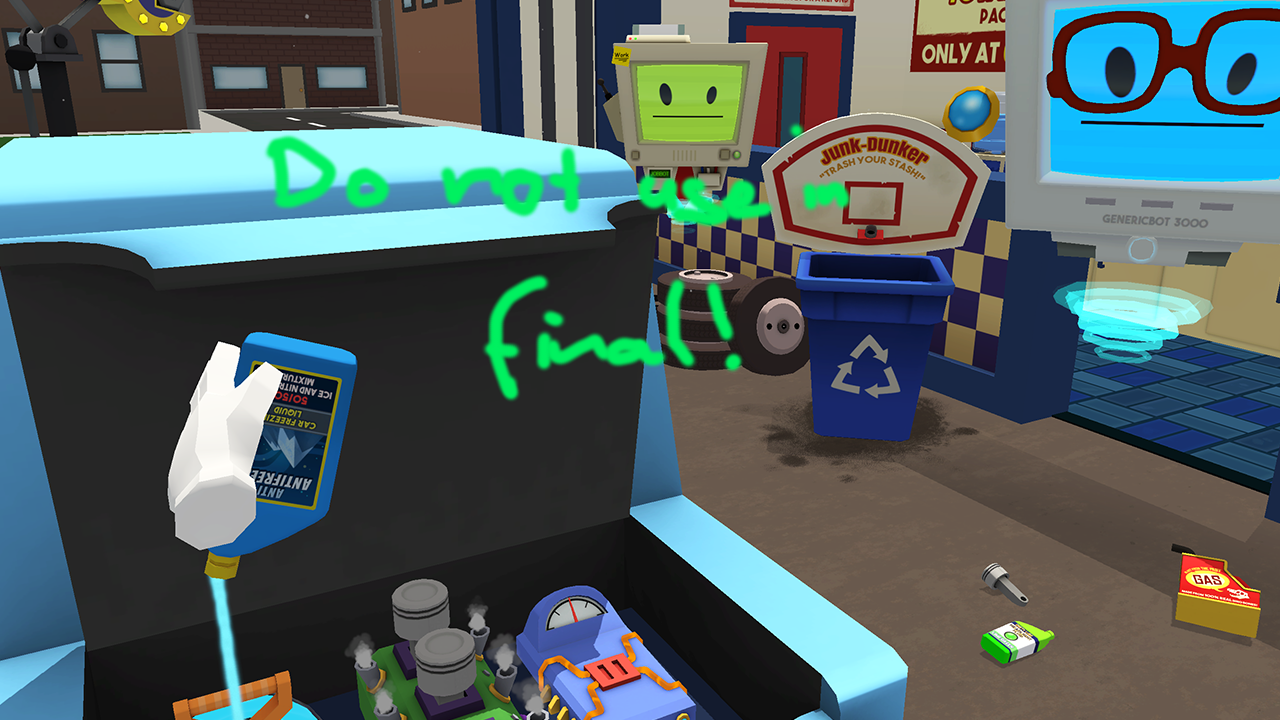
\includegraphics[width=\textwidth]{_raw_resources/job_simulator_vr.png}
		\caption{A first person, single screen output is an improvement, but is 
			hard to follow in motion.}
	\end{subfigure}
	\newline
	\begin{subfigure}[t]{.45\textwidth}
		\centering
		
\includegraphics[width=\textwidth]{_raw_resources/rickality_cctv.png}
		\caption{"Rick and Morty: Virtual Rick-Ality" allows outside observers 
			to control mounted CCTV cameras to observe the actors interaction.}
	\end{subfigure}
	\begin{subfigure}[t]{.45\textwidth}
		\centering
		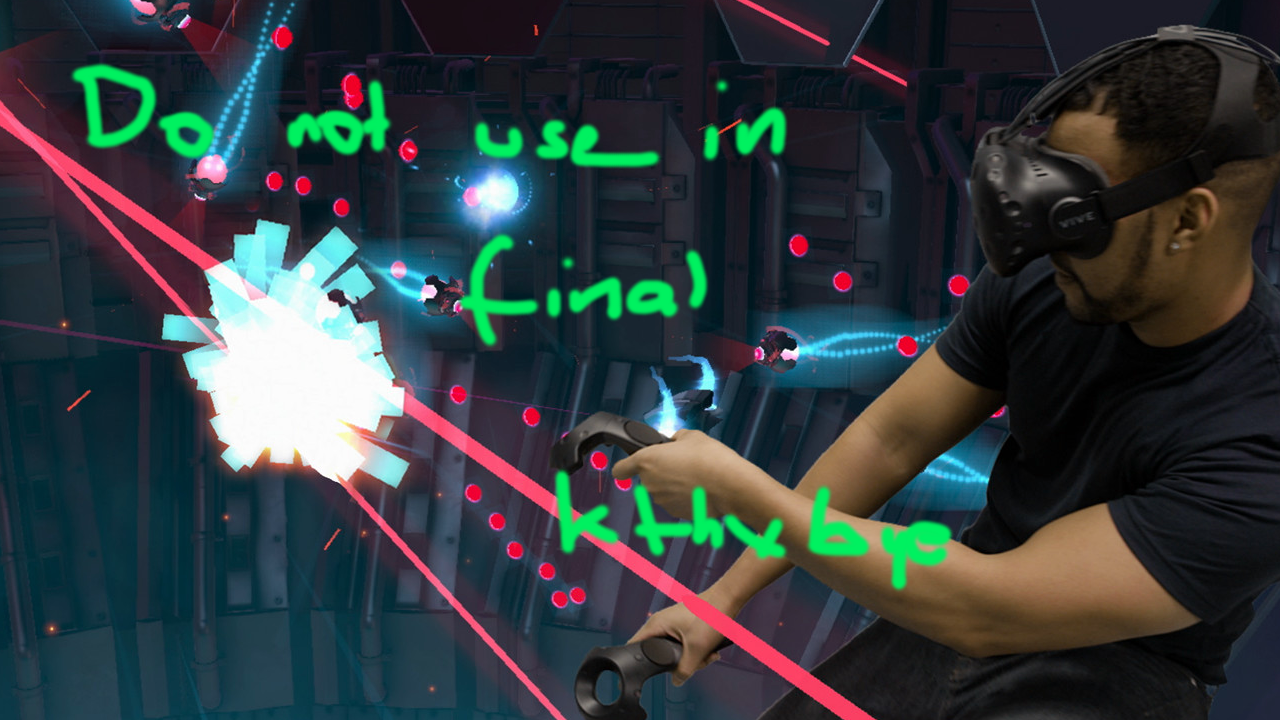
\includegraphics[width=\textwidth]{_raw_resources/the_lab_mr.png}
		\caption{Currently a screenshot of The Lab MR - but actually will be 
			one of my solution. Just gotta take some screenshots.}
	\end{subfigure}
\end{figure}

A next step was to render one eye in a full HD size and do all image 
transformations (mainly crop and distort) after it, allowing bystanders to get 
a clear first person image of the actors experience. As previously pointed out, 
this works but sometimes loses interaction context, especially when no hands 
are visible.

Then there is currently only one game, Rick and Morty: Virtual Rick-ality, that 
has an optional CCTV feature enabled, in which third persons can control a 
variety of mounted, virtual cameras and follow the actors interaction with the 
3D environment. This VR actor is then replaced with an avatar to visualize what 
he is doing.

\todo[inline]{Maybe I should pin down the timeline - how long it took for a 
next step to emerge from the medium.}

Finally there is mixed reality, where the VR actor gets placed in context of 
the virtual reality scene. This has been done previously by post-production for 
trailers and allows for a better understanding between virtual interaction and 
real actor motion. With its help it is possible to invite third person viewers 
into the VR experience in a natural way.

\section{Mixed Reality and its use cases}

\todo[inline]{There is a meeting planned to discuss A+Cs interest and use cases 
for MR - which then probably ends up in here in a summary.}

\section{Current state of Mixed Reality Production}

There have been an increasing number of presentations of mixed reality setups. 
To sort this thesis into the current scope of production environments, it is 
necessary to look at other approaches and their differences to the proposed 
solution.

\subsection{SteamVR \& Oculus SDK plugins}

Both SteamVR and Oculus SDKs supply plugins to enable mixed reality capture. 
Both system approach the problem similarly by compositing an incoming video 
stream directly at the current position of an registered camera tracker, thus 
failing to accommodate for different input latencies from the motion video 
feed. Oculus states on their manuals, that these are currently only intended 
for "for proof-of-concept, troubleshooting, and hobby use." 
\ref{oculus:2017:mr-setup}
\newline
In addition supports SteamVRs solution only video-output composition with a 4K 
HDMI output - which in turn means that the signal has to be captured on an 
external device and has to be composited on a secondary system. The 
configuration parameters are barebones at best and yielding good results is a 
matter of the best possible studio setup capture.

\subsection{Fantastic Contraption}

The game "Fantastic Contraption" from 2016 allows livestreamers to do a video 
composition for mixed reality. While this approach allows to mitigate video 
input delays it cannot have a free moving camera with an additional motion 
tracker.
\newline
"Fantastic Contraptions" trailers also show another approach by replacing the 
actor with an avatar by basically rendering a certain depth and then placing 
real world camera footage as background. With such a system any live video 
background removal is not necessary and an real world footage of the actor is 
lost. The trailer composition has been achieved in post production.

\subsection{Owlchemy Labs Mixed Reality}

Owlchemy Labs is a VR game developer located in Austin, Texas. They're working 
on VR experiments and use similar techniques discussed in this paper. Their key 
difference is visual reproduction since they're using a stereoscopic camera to 
record an actor and can reproduce the actors depth per pixel.
\newline
While Owlchemy Labs announced real time mixed reality compositing, there hasn't 
been a shipped product or update for one of their products that allows for live 
mixed reality capture.

\subsection{Apple Keynote}

Apple presented a mixed reality showcase done on their computer systems on 
their annual keynote "WWDC17". It is driven by Unreal Engine and uses also 
similar techniques as discussed in this thesis. That presentation is currently 
the best live performance of mixed reality with a high quality chroma keying, 
depth reconstruction and high fidelity graphics. There is no technical 
information available yet.